\section{Experimental Setup and Results}

\subsection{Mesh Structure and Refinement}

To evaluate the performance of the proposed hash-based remapping algorithms, we conducted experiments on 2-D mesh data sets, including structured and unstructured meshes with various levels of refinement. A central component of our evaluation is the use of Adaptive Mesh Refinement (AMR), which is widely adopted in physics simulations to allocate computational resources effectively.

In AMR, finer cells are placed in regions of interest—typically where physical gradients are high—while coarser cells cover less dynamic regions. Our experiments focus on cell-based AMR, which refines individual cells with a constraint that neighboring cells can differ by at most a factor of two in size. This allows localized refinement while keeping data structures manageable.

\subsection{Remap Scenario}

The remap operation under evaluation involves transferring data from a starting mesh to a target mesh that may have different resolution and layout due to independent AMR refinements. These remaps simulate real-world physics workflows where intermediate simulation results must be communicated between modules operating on distinct spatial decompositions.

We specifically examine how different hash strategies—perfect hash, compact hash, and hierarchical hash—perform in such remapping tasks. The objective is to test both the speed and memory footprint under increasing mesh sizes and sparsity.

\subsection{Hardware Platform}

All experiments were conducted on a high-performance computing platform featuring:
\begin{itemize}
  \item 32-core Intel Xeon CPUs (multi-core parallelism via OpenMP)
  \item NVIDIA K40 GPU (parallelism via OpenCL)
  \item Shared memory configuration for measuring inter-thread performance
\end{itemize}

The tests simulate large-scale mesh operations, running on data sets with up to 14 levels of refinement and hundreds of millions of cells.

\subsection{Performance Comparison}

Our results demonstrate that:
\begin{itemize}
  \item Hash-based methods consistently outperform kD-tree-based approaches by up to two orders of magnitude in runtime performance.
  \item Compact hashes perform best in sparse meshes due to reduced memory writes.
  \item Perfect hashes are optimal for dense, uniform meshes where collision-free mappings are easily achieved.
  \item Hierarchical hashes offer a good trade-off in mixed refinement scenarios, combining memory efficiency with reduced collision rates.
\end{itemize}

The hash methods also exhibit better scalability across architectures. On GPUs, their flat control flow and low synchronization overhead lead to efficient parallel execution, making them ideal for high-performance simulation pipelines.

\begin{figure}[h]
  \centering
  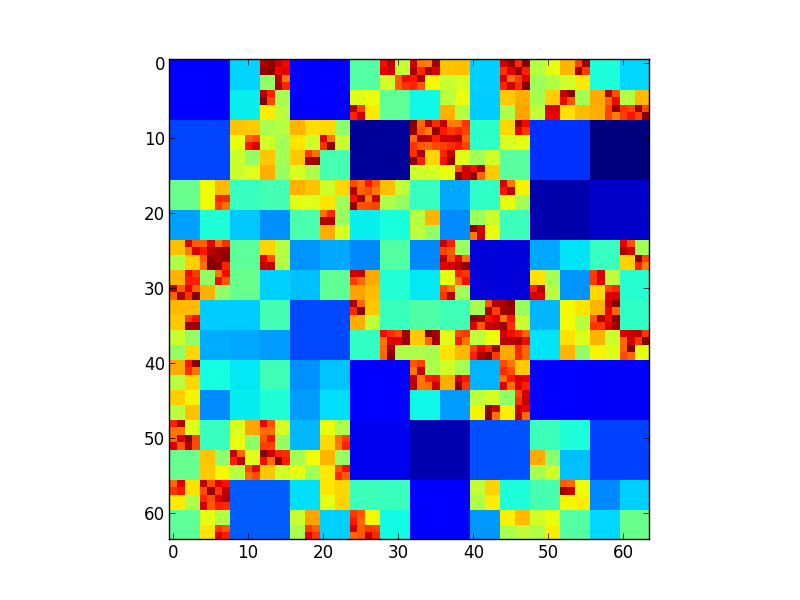
\includegraphics[width=0.75\textwidth]{./images/figure_p13_1.png}
  \caption{Performance comparison across remap methods: compact hash, perfect hash, hierarchical hash, and traditional kD-tree.}
  \label{fig:performance_comparison}
\end{figure}
